\documentclass[12pt]{beamer}
\usepackage{cmap}
\usepackage[T2A]{fontenc}
\usepackage[utf8]{inputenc}
\usepackage{ifluatex}
\usefonttheme[onlymath]{serif}
\usepackage{svg}
\usepackage{enumerate}
\usepackage{hyperref}
\usepackage{mathtools}
\setbeamertemplate{footline}[frame number]
\definecolor{beamer@darkgreen}{rgb}{0,0.6,0}
\setbeamercolor{normal text}{fg=black,bg=white}
\setbeamercolor{title}{fg=black,bg=beamer@darkgreen}
\setbeamercolor{frametitle}{fg=black,bg=beamer@darkgreen}
\setbeamercolor{background canvas}{parent=normal text}

\usepackage[english,russian]{babel}
\usepackage{graphicx}
\usepackage{listings}

\author{Катя Тузова}
\title{Машинное обучение}
\subtitle{Лекция 4. Линейные методы классификации.}
\date{}

\begin{document}	
\frame{\titlepage}

\begin{frame}\frametitle{Разбор летучки}
\end{frame}


\begin{frame}\frametitle{Постановка задачи}
$X = \mathbb{R}^n$, ${Y = \left\{ -1, + 1\right\}}$\\
${X^l = (x_i, y_i)_{i = 1}^l}$ -- обучающая выборка\\
\vspace{5mm}Найти:\\
$(n-1)$-мерную гиперплоскость, которая разделяет данные как можно лучше.
\\ \vspace{5mm}
Как можно лучше -- это как?

\end{frame}

\begin{frame}\frametitle{Пример}
\begin{figure}[htbp]
  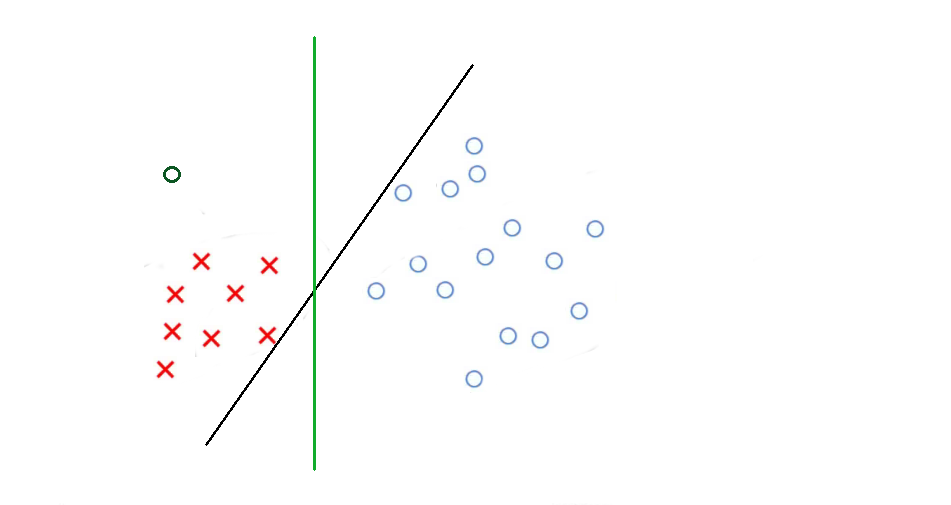
\includegraphics[height=190pt, keepaspectratio = true]{images/example}   
\end{figure}
\end{frame}

\begin{frame}\frametitle{Постановка задачи}
Как можно лучше:\\
Два разделенных класса должны лежать как можно дальше от разделяющей гиперплоскости.\\
\end{frame}

\begin{frame}\frametitle{Вопрос}
Какие есть идеи?
\end{frame}

\begin{frame}\frametitle{Пример}
\begin{figure}[htbp]
  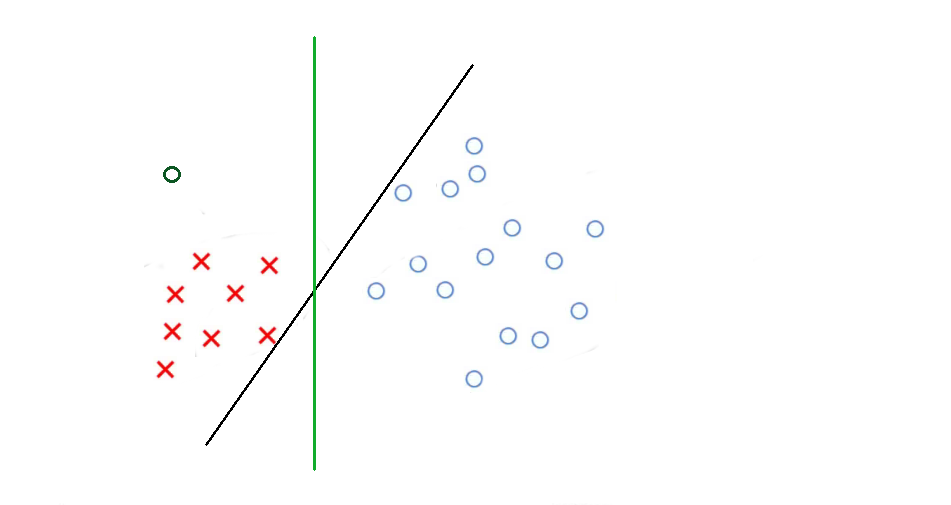
\includegraphics[height=190pt, keepaspectratio = true]{images/example}   
\end{figure}
\end{frame}


\begin{frame}\frametitle{Выпуклая оболочка}
\begin{figure}[htbp]
  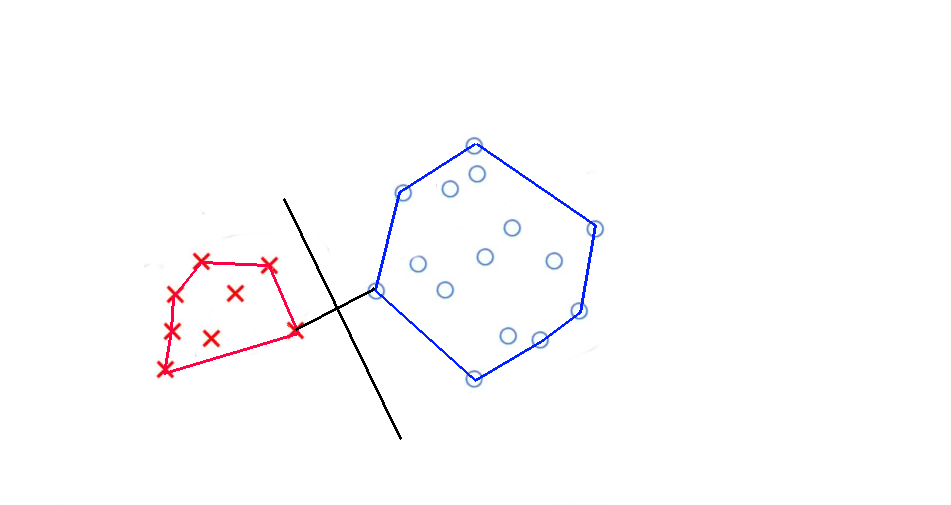
\includegraphics[height=190pt, keepaspectratio = true]{images/example1}   
\end{figure}
\end{frame}

\begin{frame}\frametitle{Выпуклая оболочка}
Выпуклой оболочкой множества $X$ называется наименьшее выпуклое множество, содержащее $X$.\\
\vspace{5mm}
Выпуклое множество — множество, содержащее вместе с любыми двумя точками соединяющий их отрезок.
\end{frame}

\begin{frame}\frametitle{Выпуклая оболочка}
Найти две ближайшие точки в выпуклых
оболочках данных, а затем провести разделяющую
гиперплоскость через середину отрезка.
\end{frame}

%\begin{frame}\frametitle{Выпуклая оболочка}
%$\min\limits_\alpha \Vert c - d \Vert^2$, где $c = \sum\limits_{y_i = 1} \alpha_ix_i$,  $d = \sum\limits_{y_i = -1} \alpha_ix_i$\\
%\vspace{5mm}
%$\sum\limits_{y_i = 1}\alpha_i = \sum\limits_{y_i = -1}\alpha_i = 1$, $\alpha_i \geq 0$\\
%\vspace{5mm}
%Задачу можно решать общими оптимизационными алгоритмами.
%\end{frame}

\begin{frame}\frametitle{Опорная гиперплоскость}
\end{frame}

\begin{frame}\frametitle{Построение разделяющей поверхности}
${X^l = (x_i,y_i)_{i = 1}^l}$ -- обучающая выборка\\ 
${Y=\left\{-1,+1\right\}}$\\
\vspace{5mm}
Задача:\\
Построить алгоритм классификации ${a(x,w) = sign f(x,w)}$\\\vspace{5mm}
${f(x,w)}$ -- разделяющая функция\\
$w$ -- вектор параметров, $w \in \mathbb{R}^l$
\end{frame}

\begin{frame}\frametitle{Опорная гиперплоскость}
Гиперплоскость называется опорной для множества точек
$X$, если все точки из $X$ лежат по одну сторону от этой гиперплоскости.\\\vspace{5mm}
${f(x,w) = \langle x, w\rangle - w_0 = 0}$\\
\vspace{5mm}
Расстояние от точки до гиперплоскости:
$\frac{\vert f(x,w) \vert}{\Vert w \Vert}$
\end{frame}


\begin{frame}\frametitle{Построение разделяющей поверхности}
Как оценить надежность классификатора?
\end{frame}

\begin{frame}\frametitle{Минимизация зазора}
${f(x,w) = 0}$ -- разделяющая поверхность\\
${M_i(w) =y_if(x_i,w)}$ -- отступ объекта $x_i$\\
${M_i(w)<0}$ $\Rightarrow$ алгоритм $a(x,w)$ ошибается на $x_i$
\end{frame}

%\begin{frame}\frametitle{Максимизиция отступа}
%Идея:\\
%Максимизировать отступ между
%двумя параллельными опорными плоскостями, а затем
%провести параллельную им плоскость на равных расстояниях.\\
%\vspace{5mm}
%Как посчитать расстояние от точки до гиперплоскости?
%\end{frame}

%\begin{frame}\frametitle{Постановка задачи}
%Задача классификации:
%$X = \mathbb{R}^n$, ${Y = \left\{ -1, +1\right\}}$\\
%${X^l = (x_i, y_i)_{i = 1}^l}$ -- обучающая выборка\\
%\vspace{5mm}
%Найти:\\
%$w \in \mathbb{R}^n, w_0 \in \mathbb{R}$ -- параметры алгоритма классификации\\
%${a(x, w) = sign(\langle x, w\rangle + w_0) }$
%\end{frame}

\begin{frame}\frametitle{Минимизация эмпирического риска}
Число ошибок на обучающей выборке:\\
\vspace{5mm}
${Q(w) = \sum\limits_{i=1}^l \left[ M_i(w) < 0 \right] \rightarrow \min\limits_w }$\\
\vspace{3mm}
${Q(w)}$ -- функционал качества\\
\vspace{5mm}
Но так мы учитываем только результат классификации и теряем информацию насколько ${i}$-й объект был надежен.\\
\vspace{3mm}
Как сохранить информацию?

\end{frame}

\begin{frame}\frametitle{Минимизация эмпирического риска}
${Q(w) = \sum\limits_{i=1}^l \left[ M_i(w) < 0 \right] \leq}$\\ \vspace{3mm}
${\leq \widetilde{Q}(w) = \sum\limits_{i=1}^l \mathcal{L}(M_i(w)) \rightarrow \min\limits_w }$\\\vspace{3mm}
$\mathcal{L}$ -- функция потерь, невозрастающая, неотрицательная.\\ 
\end{frame}

\begin{frame}\frametitle{Примеры $\mathcal{L}$}
\begin{figure}[htbp]
  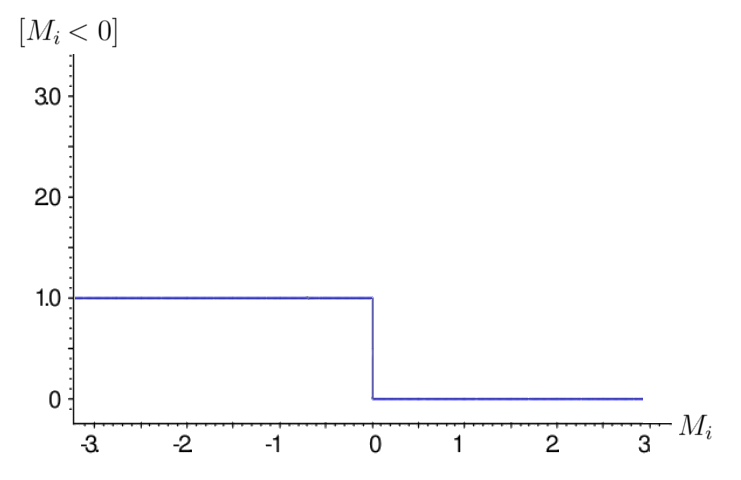
\includegraphics[height=160pt, keepaspectratio = true]{images/l1}   
\end{figure}
\end{frame}

\begin{frame}\frametitle{Примеры $\mathcal{L}$}
\begin{figure}[htbp]
  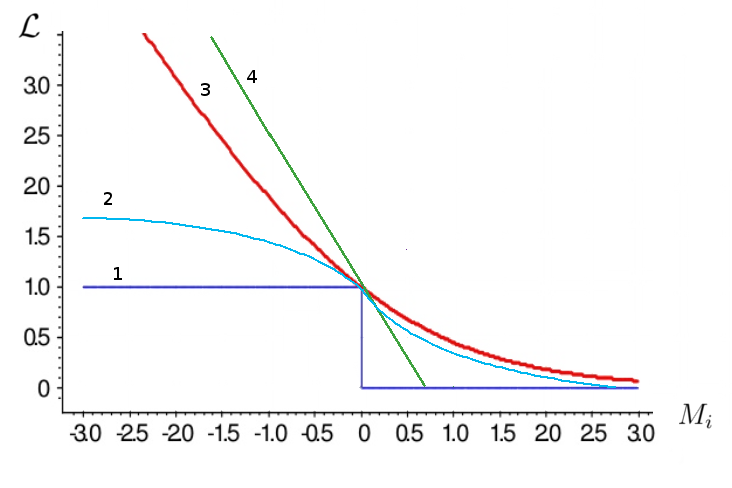
\includegraphics[height=160pt, keepaspectratio = true]{images/l}   
\end{figure}
\begin{enumerate}
\item $V(M) = (1-M)_+$ -- кусочно-линейная
\item $L(M) = \log_2(1+e^{-M})$ -- логарифмическая
\item $H(M) = (-M)_+$ -- кусочно-линейная
\item $S(M) = 2(1+e^M)^{-1}$ -- сигмоидная
\end{enumerate}
\end{frame}

\begin{frame}\frametitle{Линейный классификатор}
$f_j: X \rightarrow \mathbb{R}$, $j = 1,\dots, n$\\
\vspace{3mm}
$a(x, w) = sign(\sum\limits_{j=1}^n w_jf_j(x) - w_0)$\\
\vspace{3mm}
$w_j \in \mathbb{R}$ -- веса признаков\\
\end{frame}

\begin{frame}\frametitle{Линейный классификатор}
$a(x, w) = sign(\sum\limits_{j=1}^n w_jf_j(x) - w_0)$\\
\vspace{3mm}
Введем константный признак $f_0 \equiv -1$:\\
\vspace{3mm}
$a(x, w) = sign(\langle w, x\rangle)$\\
\vspace{3mm}
Отступ:\\
$M_i(w) = \langle w, x_i\rangle y_i$
\end{frame}


\begin{frame}\frametitle{Линейный классификатор}
\begin{figure}[htbp]
  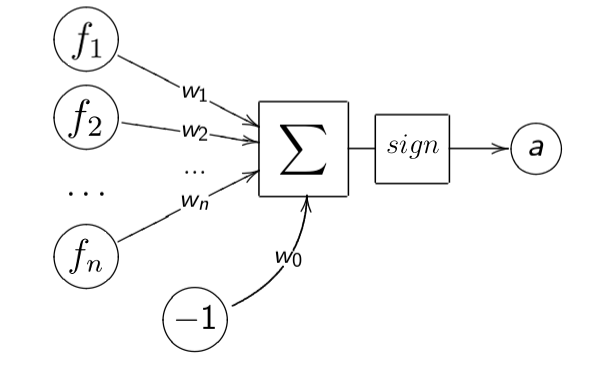
\includegraphics[height=160pt, keepaspectratio = true]{images/neuron}   
\end{figure}
\end{frame}

%Численный метод оптимизации
\begin{frame}\frametitle{Метод градиентного спуска}
$w^{(0)} $ -- начальное приближение\\
\vspace{3mm}
$w^{(t+1)} =  w^{(t)} - \eta \bigtriangledown Q(w^{(t)})$\\
\vspace{3mm}
$\bigtriangledown Q(w) = (\frac{\partial Q(w)}{\partial w_j})_{j=0}^n$\\
\vspace{3mm}
$\eta$ -- градиентный шаг (темп обучения)\\
\vspace{3mm}
$w^{(t+1)} =  w^{(t)} - \eta \sum\limits_{i=1}^l \mathcal{L}'(\langle w^{(t)}, x_i\rangle y_i)x_iy_i$\\
\end{frame}

\begin{frame}\frametitle{В чем проблема?}
$w^{(t+1)} =  w^{(t)} - \eta \sum\limits_{i=1}^l \mathcal{L}'(\langle w^{(t)}, x_i\rangle y_i)x_iy_i$\\
\end{frame}

\begin{frame}\frametitle{В чем проблема?}
$w^{(t+1)} =  w^{(t)} - \eta \sum\limits_{i=1}^l \mathcal{L}'(\langle w^{(t)}, x_i\rangle y_i)x_iy_i$\\
\vspace{5mm}
Очень медленно сходится.
\end{frame}

\begin{frame}\frametitle{Метод стохастического градиента}
$w^{(t+1)} =  w^{(t)} - \eta \sum\limits_{i=1}^l \mathcal{L}'(\langle w^{(t)}, x_i\rangle y_i)x_iy_i$\\
\vspace{5mm}
Давайте брать $(x_i, y_i)$ по одному и сразу обновлять вектор весов
\end{frame}


\begin{frame}\frametitle{Алгоритм}
Input: $X^l$, $\eta$, $\lambda$\\
Output: $w_0, w_1, \dots, w_n$\\
\vspace{3mm}
Инициализировать: $w_j$, $j=0,\dots, n$\\
\hspace{35mm} ${Q}(w) = \sum\limits_{i=1}^l \mathcal{L}(\langle w, x_i \rangle y_i)$\\
Повторить пока $Q$ и/или $w$ не стабилизируются:\\
\hspace{5mm} выбрать $x_i$ из $X^l$ случайным образом\\
\hspace{5mm} Потеря: $\varepsilon_i = \mathcal{L}(\langle w, x_i \rangle y_i)$\\
\hspace{5mm} Градиентный шаг: $w =  w - \eta \mathcal{L}'(\langle w, x_i\rangle y_i)x_iy_i$\\
\hspace{5mm} Оценить $Q = (1-\lambda)Q + \lambda \varepsilon_i$
\end{frame}


\begin{frame}\frametitle{Учет ошибки $\varepsilon_i$ в алгоритме}
\begin{figure}[htbp]
  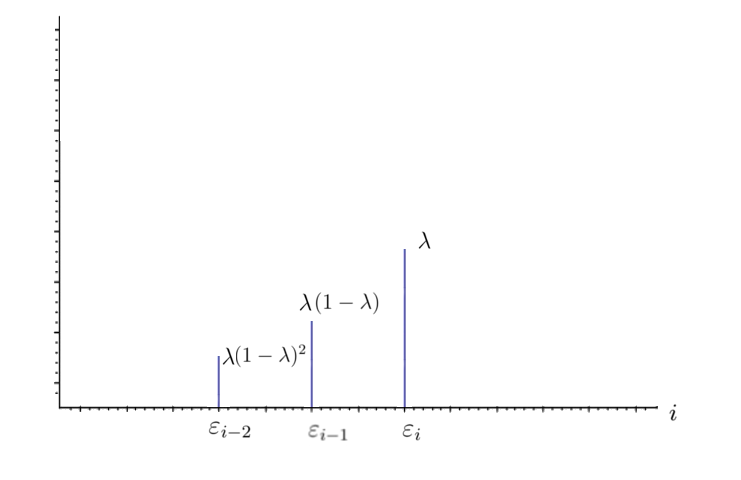
\includegraphics[height=160pt, keepaspectratio = true]{images/l2}   
\end{figure}
\end{frame}

\begin{frame}\frametitle{Вопрос}
Чего не хватает?
\end{frame}

\begin{frame}\frametitle{Вопрос}
Как выбрать параметр $\lambda$?
\end{frame}

\begin{frame}\frametitle{Эмпирическое правило для выбора $\lambda$}
$\lambda = \frac{1}{k}$, где $k$ -- количество объектов, по которым хотим усреднять функционал.
\end{frame}

\begin{frame}\frametitle{Вопрос}
Что значит -- "пока $Q$ и/или $w$ не стабилизируются"?
\end{frame}

\begin{frame}\frametitle{Зависимость $Q$ от номера итерации}
\begin{figure}[htbp]
  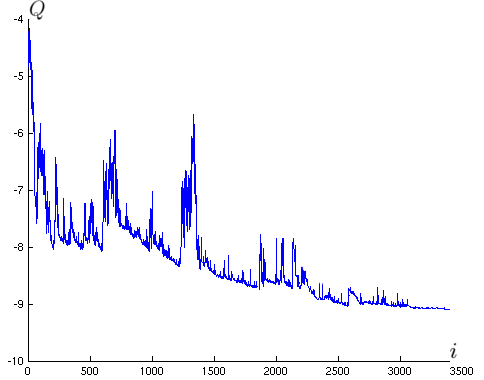
\includegraphics[height=160pt, keepaspectratio = true]{images/stochastic_gradient}   
\end{figure}
\end{frame}

\begin{frame}\frametitle{Актуальные вопросы}
\begin{itemize}
\item[--] Инициализация весов
\item[--] Порядок предъявления объектов
\item[--] Выбор величины шага
\end{itemize}
\end{frame}

\begin{frame}\frametitle{Инициализация весов}

\end{frame}

\begin{frame}\frametitle{Инициализация весов}
\begin{itemize}
\item[--] $w_j = 0$, j = 1, \dots, n
\item[--] $w_j = random(-\frac{1}{2n}, \frac{1}{2n})$ -- небольшие случайные значения
\item[--] $w_j = \frac{\langle y, f_j \rangle}{\langle f_j, f_j \rangle}$, $f_j = (f_j(x_i))_{i = 1}^n$
\item[--] Обучение по небольшой случайной подвыборке объектов
\item[--] Многократный запуск из разных случайных начальных приближений
\end{itemize}

\end{frame}

\begin{frame}\frametitle{Порядок предъявления объектов}

\end{frame}

\begin{frame}\frametitle{Порядок предъявления объектов}
\begin{itemize}
\item[--] Попеременно брать объекты из разных классов
\item[--] Чаще брать те объекты, на которых была допущена большая ошибка
\item[--] Вообще не брать "хорошие" объекты с $M_i > \mu_+$
\item[--] Вообще не брать выбросы с $M_i < \mu_-$
\end{itemize}
\end{frame}

\begin{frame}\frametitle{Выбор величины шага}

\end{frame}

\begin{frame}\frametitle{Выбор величины шага}
Для выпуклых функций:
\begin{itemize}
\item[--] $\eta_t \rightarrow 0$
\item[--] $\sum\limits_{t = 1}^\infty \eta_t = \infty$
\item[--] $\sum\limits_{t = 1}^\infty \eta_t^2 < \infty$
\end{itemize}
Метод скорейшего градиентного спуска:
\begin{itemize}
\item[--] 
$Q(w - \eta \bigtriangledown Q(w)) \rightarrow \min\limits_{\eta}$
\end{itemize}
Пробные случайные шаги
\end{frame}

\begin{frame}\frametitle{Плюсы и минусы}
\begin{itemize}
\item[+] Легко реализовать
\item[+] Легко обобщить на разные $f$, $\mathcal{L}$
\item[+] Не обязательно брать все элементы выборки для обучения
\end{itemize}
\begin{itemize}
\item[--] Возможна медленная сходимость
\item[--] Застревание в локальных минимумах
\item[--] Подбор параметров
\item[--] Проблема переобучения
\end{itemize}
\end{frame}

\begin{frame}\frametitle{Проблема переобучения}
Почему случается переобучение?
\end{frame}

\begin{frame}\frametitle{Проблема переобучения}
\begin{itemize}
\item[--] Слишком мало объектов; слишком много признаков
\item[--] Линейная зависимость признаков
\end{itemize}
\end{frame}

\begin{frame}\frametitle{Как заподозрить?}
\begin{itemize}
\item[--] Слишком большие веса $\Vert w \Vert$
\item[--] Неустойчивость $a(x,w)$
\item[--] 
\end{itemize}
\end{frame}

\begin{frame}\frametitle{Решение}
\begin{itemize}
\item[--] Сокращение весов
\item[--] Ранний останов
\item[--] 
\end{itemize}
\end{frame}

\begin{frame}\frametitle{Сокращение весов}

\end{frame}

\begin{frame}\frametitle{Принцип максимума правдоподобия}

\end{frame}

\begin{frame}\frametitle{Регуляризация?}

\end{frame}

\begin{frame}\frametitle{ROC-кривая}

\end{frame}

\begin{frame}\frametitle{Построение ROC-кривой}

\end{frame}
\end{document}
